%\documentclass[letterpaper,peerreview,12pt,compsoc,draftcls]{IEEEtran}
%\documentclass[10pt,twocolumn,letterpaper]{article}
\documentclass[letterpaper]{article}

%
% Final Checklist TODO XXX 
% - Spellcheck
% - check xxx's todo's etc
%
%\usepackage{ruler}
%\usepackage{cvpr}
%\usepackage{iccv}
\usepackage{times}
\usepackage{epsfig}
\usepackage{graphicx}
\usepackage{amsmath}
\usepackage{amssymb}
%\usepackage{amsthm}
\usepackage{mathtools,empheq}
\usepackage[tight,footnotesize]{subfigure}
%\usepackage{caption}
\usepackage{verbatim}
\usepackage{color}
\usepackage{nomencl}
\usepackage[nocompress]{cite}
\usepackage[pagebackref=true,breaklinks=true,letterpaper=true,colorlinks,bookmarks=false]{hyperref}
\usepackage{algorithm}
\usepackage{enumerate}
\usepackage{multirow}
\usepackage[width=122mm,left=12mm,paperwidth=146mm,height=193mm,top=12mm,paperheight=217mm]{geometry}


\newcommand{\intinf}{\int_{-\infty}^{\infty}}
\newcommand{\argmin}{\operatornamewithlimits{argmin}}

\newcommand{\grad}{\nabla}
\newcommand{\slant}{\sigma}
\newcommand{\R}{\mathbb{R}} % the reals
\newcommand{\skewm}[1]{{#1}_\times}

\renewcommand{\vec}[1]{\mathbf{#1}}

\newcommand{\lbar}{\overline}

\newcommand{\id}{\text{\emph{I}}}
\newcommand{\ransac}{\textsc{ransac}}
\newcommand{\sift}{\textsc{sift}}
\newcommand{\klt}{\textsc{klt}}
\newcommand{\svd}{\textsc{svd}}
\newcommand{\sfm}{\textsc{sfm}}


\newtheorem{thm}{Theorem}
\newtheorem{lem}[thm]{Lemma}

%\newtheorem{theorem}{Theorem}[section]
%\newtheorem{corollary}[theorem]{Corollary}
\newtheorem{corolary}[theorem]{Corollary}
%\newtheorem{proposition}[theorem]{Proposition}
%\newtheorem{lemma}[theorem]{Lemma}

%\theoremstyle{definition}
%\newtheorem{definition}{Definition}
%\newtheorem{remark}{Remark}[section]
\newtheorem{assumption}{Assumption}[section]
%\newtheorem{problem}{Problem}[section]
%\newtheorem{question}{Question}[section]
%\newtheorem{property}{Property}
\newtheorem{transformation}{Transformation}

\numberwithin{equation}{section}

\newcommand{\Gama}{\boldsymbol{\Gamma}}
\newcommand{\gama}{\boldsymbol{\gamma}}
\newcommand{\bsigma}{\boldsymbol{\sigma}}
%\newcommand{\Gama}{\Gamma}
%\newcommand{\gama}{\gamma}
\newcommand{\T}{\boldsymbol{T}}
\newcommand{\N}{\mathbf{N}}
\newcommand{\NSurface}{\mathbf{N}}
\newcommand{\Nlocal}{\overline{\N}} % normal in local coordinates
\newcommand{\balpha}{\boldsymbol{\alpha}}
\newcommand{\tDt}{t+\Delta t}
\newcommand{\bpsi}{\boldsymbol{\boldsymbol{\psi}}}
\newcommand{\bp}{\mathbf p}
\newcommand{\deldt}[1]{\frac{\partial#1}{\partial t}}
\newcommand{\ddt}[1]{\frac{d #1}{dt}}
\newcommand{\delds}[1]{\frac{\partial#1}{\partial s}}
\newcommand{\mybar}[1]{\overline{#1}}
\newcommand{\norm}[1]{\|#1\|}
\newcommand{\I}{\mathbf{I}}
\newcommand{\brho}{\boldsymbol{\rho}}
\newcommand{\lightrgb}{\boldsymbol{l}}
\newcommand{\B}{\boldsymbol{B}}
\renewcommand{\t}{\boldsymbol{t}}
\newcommand{\n}{\boldsymbol{n}}
\renewcommand{\b}{\boldsymbol{b}}
\newcommand{\e}{\boldsymbol{e}}
\newcommand{\f}{\boldsymbol{e}_3}
\newcommand{\ff}{\mathbf{f}}
\newcommand{\hf}{\boldsymbol{\hat{f}}}
\newcommand{\g}{\boldsymbol{g}}
\newcommand{\G}{\boldsymbol{G}}
\newcommand{\bc}{\boldsymbol{c}}
\newcommand{\Curve}{\Gamma}
%\newcommand{\X}{\boldsymbol{X}}
%\newcommand{\x}{\boldsymbol{x}}
\newcommand{\X}{\mathbf{X}}
\newcommand{\x}{\mathbf{x}}
\newcommand{\tilx}{\tilde x}
\newcommand{\tily}{\tilde y}
\newcommand{\tilgama}{\tilde \gama}
\newcommand{\ugama}{\hat{\gama}} %unit gama
\newcommand{\br}{\bar r}
\newcommand{\Kc}{\mathbf K_c}
\newcommand{\Kim} {\mathcal K_{im}}
\newcommand{\lepi}{\mathbf r}
\newcommand{\itan}{\tan^{-1}}
\newcommand{\uu}{\xi}
\newcommand{\buu}{\bar \uu}
\newcommand{\bvv}{\bar \vv}
\newcommand{\vv}{\eta}
\newcommand{\VV}{\mathbf{V}} % translational velocity
\newcommand{\VVspeed}{V} % translational velocity
\newcommand{\field}{\boldsymbol\chi}
\newcommand{\ufield}{\hat{\boldsymbol{\chi}}}
\newcommand{\fieldc}{\chi} % field component
\newcommand{\transl}{\mathcal{T}}
\newcommand{\rot}{\mathcal{R}}
\newcommand{\albedo}{\alpha}
\newcommand{\depth}{\rho}      % depth as z
\newcommand{\udepth}{{\hat{\rho}}} % depth along ray
\newcommand{\ttransl}{\T} % translation tangent
\newcommand{\surface}{\mathcal{M}} % surface/manifold
\newcommand{\surf}{\mathcal{M}} % surface/manifold short
\newcommand{\jacm}{\mathtt{J}} % Jacobian matrix
\newcommand{\xbar}{\bar x}
\newcommand{\ybar}{\bar y}
\newcommand{\zbar}{\bar z}

\newcommand{\bdelta}{\boldsymbol \delta}
%\newcommand{\X}{\boldsymbol{X}}
%\newcommand{\x}{\boldsymbol{x}}
%\newcommand{\X}{\mathbf{X}}
%\newcommand{\x}{\mathbf{x}}
\newcommand{\boldu}{\mathbf{u}}
\newcommand{\boldv}{\mathbf{v}}
\newcommand{\boldw}{\mathbf{w}}
% The following are not very good constructs it seems. Better to use just
% \begin{bmatrix}..\end{\bmatrix}
\newcommand{\datsqbr}[2][rrrrrrrrrrrrrrrrrrrrrrrrrrrrrrrrrrrr]{\left[
\begin{array}{#1}
#2\\
\end{array}
\right]
}
\newcommand{\tgtveloc}{\tilde\alpha} % real tangential velocity
\newcommand{\trace}{\text{trace}\,}
\newcommand{\benx}{x} % ben's aux. variable in da calibration paper

\newcommand{\ie}{{\it i.e.}}
\newcommand{\etc}{{\it etc}}
\newcommand{\eg}{{\it e.g.}}
\newcommand{\wrt}{{\it w.r.t. }}
\newcommand{\etal}{{\it et.~al.}}


\usepackage{url}
\usepackage{graphicx}
\usepackage[tight,footnotesize]{subfigure}
\usepackage{color}
\usepackage{verbatim}
\usepackage{multirow}
\usepackage[pagebackref=true,breaklinks=true,letterpaper=true,colorlinks,bookmarks=false]{hyperref}

%%%%%%%%%%%%%%%%%%%%%%%%%%%%%%%%%%%%%%%%
% You have two versions of the macro
% \draftnote{My note}. The first version puts notes (e.g. My note in the example)
% into the margin of your document. The second formats the note as nothing. You
% 'comment out' the version of the macro you don't want (using a % at the
% beginning of the line).
%\newcommand{\draftnote}[1]{\marginpar{\tiny\raggedright\textsf{\hspace{0pt}#1}}}
\newcommand{\draftnote}[1]{\marginpar{\tiny\raggedright\textsf{\hspace{0pt}#1}}}
%\newcommand{\draftnote}[1]{}

% This one is just for the comments for in-line text.
\newcommand{\indraftnote}[1]{\textcolor{blue}{\texttt{\footnotesize[#1]}}}
\newcommand{\todo}[1]{\indraftnote{todo: #1}}
%\newcommand{\indraftnote}[1]{}


\begin{document}
\title{%
AA Distributed Software Development Methodology
}

\author{%
Renato~Fabbri \and Ricardo~Fabbri \and Vilson Vieira \and Alexandre Negrao \and Lucas Zambianchi
\and Marcos Mendonca
}

\maketitle
%\thispagestyle{empty}


\begin{abstract}
Algorithmic Autoregulation is a new self-regulating methodology for coordinating
distributed teamwork,  based on collaboration and
individual merit. Team members take on an egalitarian role, and stay
voluntarily logged into so-called AA sessions for part of their time (e.g.,
2h/day), during which they check for open tickets and microblog periodical
"tweets" or status messages they wish to share about their activity with the
team. These status logs are publicly aggregated and are peer-validated,
as in code review, and a public videolog is recorded summarizing daily experiences.
This methodology is well-suited for increasing the efficiency of distributed
teams through asynchronous on-demand communication, reducing the need for
central management, unproductive meetings or time-consuming reports.  The AA
methodology also legitimizes the activities of a distributed software team.  It
thus enables entities to have a solid means to fund these activities, allowing
for new and concrete business models to emerge for very distributed software
development.  
\end{abstract}



\section{Introduction}

One of the defining features of modern times is the widening
geographical distribution of software teams~\cite{last2003} creating
what is called Global Software Development (henceforth
GSD)~\cite{german2003}. An example is the free software
movement. Projects and institutions like Mozilla Foundation has several
employees and thousands of voluntary developers distributed across
many countries. The same is true for GNOME~\cite{german2003}, OpenBSD,
MySQL or Apache Software Foundation, to cite just a few of the most active
projects.\footnote{Ohloh, the open source network, have a more complete
  and constantly updated list of the most active projects on-line at
  \url{www.ohloh.net}} Along the free and open software
projects, GSD is growing popularity in every niche of the software
industry as a whole, even on those distributing their software with
proprietary licenses. This phenomenon is attributed to a variety of factors
such as a larger labor pool, natural globalization of software companies
and foundations or even the premise of cheaper cost of
production~\cite{komi2005}.

Despite the advantages of GCD, we have noticed how
difficult it is to coordinate and fund free software on a larger scale
than currently available, when teams are very heterogeneous containing
not only volunteers and very experienced developers, but also
contractors and freelancers from different backgrounds and cultures. Our observations
are founded on the factors suggested by Carmel~\cite{carmel1999} as
main difficulties for GCD: distance, time and cultural differences. In
the case of free or open software projects, all these factors are
involved.

Another problem faced by modern software companies and other
collectives are frequent ineffective meetings, which are seldom
focused to the interest to any attendant. The result is that it has
become the norm to participate in too many meetings with the ``laptop
open'', which can be un-productive. Software developers
like to code, to be productive, to have their hands on their project,
to do what they are best at. They dislike to forcibly stop for meetings
or to do other bureaucratic activities such as writing lengthy reports to
justify their funding.~\cite{Thompson:Wired:2012}
%\todo{ler mais. cacm, etc}

In this paper we propose the AA methodology and an associated software system
for coordinating distributed team work, tackling the disadvantages
of GSD. Team members take on an egalitarian role, and stay
voluntarily \textit{logged} in the system for part of their time
(e.g.\ 2 hours per day), during which they log a periodical short text
sentence or \emph{microlog} --- similar to a `tweet' from Twitter --- as the
status of their activity. Logging is carried out using an easy a series of
available UI's: unix shell
commands, native GUI or web page, conventional social network posts, or chat messages to a log bot
listening to IRC, GTalk, G+, and others.  These ``microblog sentences'' are publicly aggregated and validated by other
team members. Through AA, we have a methodology and an associated system to help
implement and validate the activities of a distributed software team. It implicitly
legitimizes financial support for the expansion of the activity of the developer
team. The AA methodology is specially useful for coordinating distributed and
decentralized team work, providing effective means to asynchronously update
different team members without the need for synchronous unproductive meetings.

%\todo{alerts work for greater consciousness of time}
%\todo{Integrate notes from Ricardo+Renato april 15/16 meeting}
%\todo{integrate IRC chat notes}

A brief overview of current work on GSD methodologies related to
AA is presented in Section~\ref{related-work}, while in
Section~\ref{aa-methodology} we describe the most relevant
characteristics of the AA methodology followed by the description of
our experience using AA in a team of 9 paid developers 
% nao era mais de 9?
since July 2011. In Section~\ref{conclusions} we draw some final
conclusions and indicate future possibilities for the
practical use of AA in other types of software developers teams or
organizations working on non-software distributed activities.

\indraftnote{
A very good article on the value of asynchronous communication for personal
and group productivity, related to the key necessity of having moments of
introversion to avoid daily pressures of forced socialization. The way we work
on the digital age enables people to be very productive, the article also
mentions linux as a hallmark example~\cite{Thompson:Wired:2012}
}

\indraftnote{TODO: cite CIA.vc bot stuff}

\section{Related Work}
\label{related-work}

%% aqui tomei como ponto de vista as metodologias associadas a GSD
%% (Global Software Development) que considero foco do AA, e sua
%% principal vantagem

%\todo{survey other methodologies such as agile etc}
%\todo{probably a good source http://agilemanifesto.org/}

There has been a large amount of research done in the area of
methodologies to deal with distributed teams of developers. We are
focusing in GSD here, however some principles involved on those
methodologies could be used on smaller teams of developers working in
the same place, time and with minor cultural differences. Moreover we
generally think on ``distributed development'' being global which is
not totally true. We even applied AA to a team that work at the same
city but on different times (more details on
Section~\ref{results}). Even smaller groups of developers working on
the same building could use GSD methodologies. A thorough survey of
these methodologies is beyond the scope of this paper. Here we present
a brief overview.

Various methodologies for GSD were built around the factors that
affect distributed team works, proposed by Carmel~\cite{carmel1999}
and comprising three distances: geographical, cultural and
temporal. 

First, geographical distance handicaps ($i$) \emph{coordination}, the act of
integrating all the tasks distributed between units~\cite{carmel2001}; ($ii$)
\emph{control}, or the process to maintain specific goals, policies or quality
levels; and ($iii$) \emph{communication}. All those factors are correlated, \eg,
a team needs to have clear communication to work on tasks of a specific problem.  

Second, cultural distance encompasses differences on organizational and
natural culture. Spoken language, unit and ethnic values are common
forms of such distance. Some companies prefer to allocate development
units in foreign locations with minimal cultural distance (\eg, an
American company may prefer Ireland due to spoken language
similarity~\cite{carmel2001}). Third, the temporal distance that
hampers synchronous communications like telephone or
videoconferences. Units of developers working on different time-zones
are concerned with managing of their agenda guided by this temporal
distance.

Targeting geographical distance, Carmel~\cite{carmel2001} suggests a
strategy to reduce intensive collaboration. His approach divides the
whole software life-cycle into levels of complexity. Each level has a
degree of collaboration. For example, some developers working on a
project with high collaboration level should use the follow-the-sun
approach: when concluding the work day, they pass their work to the
team working on another time-zone. Other tactics are suggested by the
same author to deal with the three distances, such as separating foreign
units of developers in time-zone bands.

Battin~\etal~\cite{battin2001} propose and discuss their
experiments using specific methodologies created for the distributed
development centers from Motorola (at the time having 25+
software development centers worldwide). These methodologies included
constant communication with critical units, incremental integration
and schedules based on time-zones distributed to developers on 6
countries from 3 continents.

In considering free software projects instead of companies,
similar factors are present and specialized methodologies
arise. German~\cite{german2003} provides a concise review of
the methodologies used by the GNOME project, one of the most active of all free
software projects. The manuscript is centered on the software architecture. It
begins by explaining that GNOME is separated into modules (76 on version 2.4, to be
precise) and each module has one maintainer who divides his modules into
separate parts in which other developers can work on independent tasks, along
other responsibilities. As in other free software projects, all 
development was done using a \emph{bugtracker} for bug and issue management,
mail lists and Internet Relay Chat (IRC) for discussion and communication and a
version control system like Git or Mercurial. Periodical (commonly yearly)
conferences like GUADEC is common on free and open source projects for
face-to-face meetings and is based on a different place each time.


\section{The AA Methodology}
\label{aa-methodology}

Some of the strategies for GSD mentioned on the previous section are based on complex methodologies
and many were built for a specific company or software
center. We propose an alternative methodology based on a simple
idea: small working sessions logged by a computational
tool. Figure~\ref{fig:mm} summarizes our methodology.

\begin{figure}
\begin{center}
   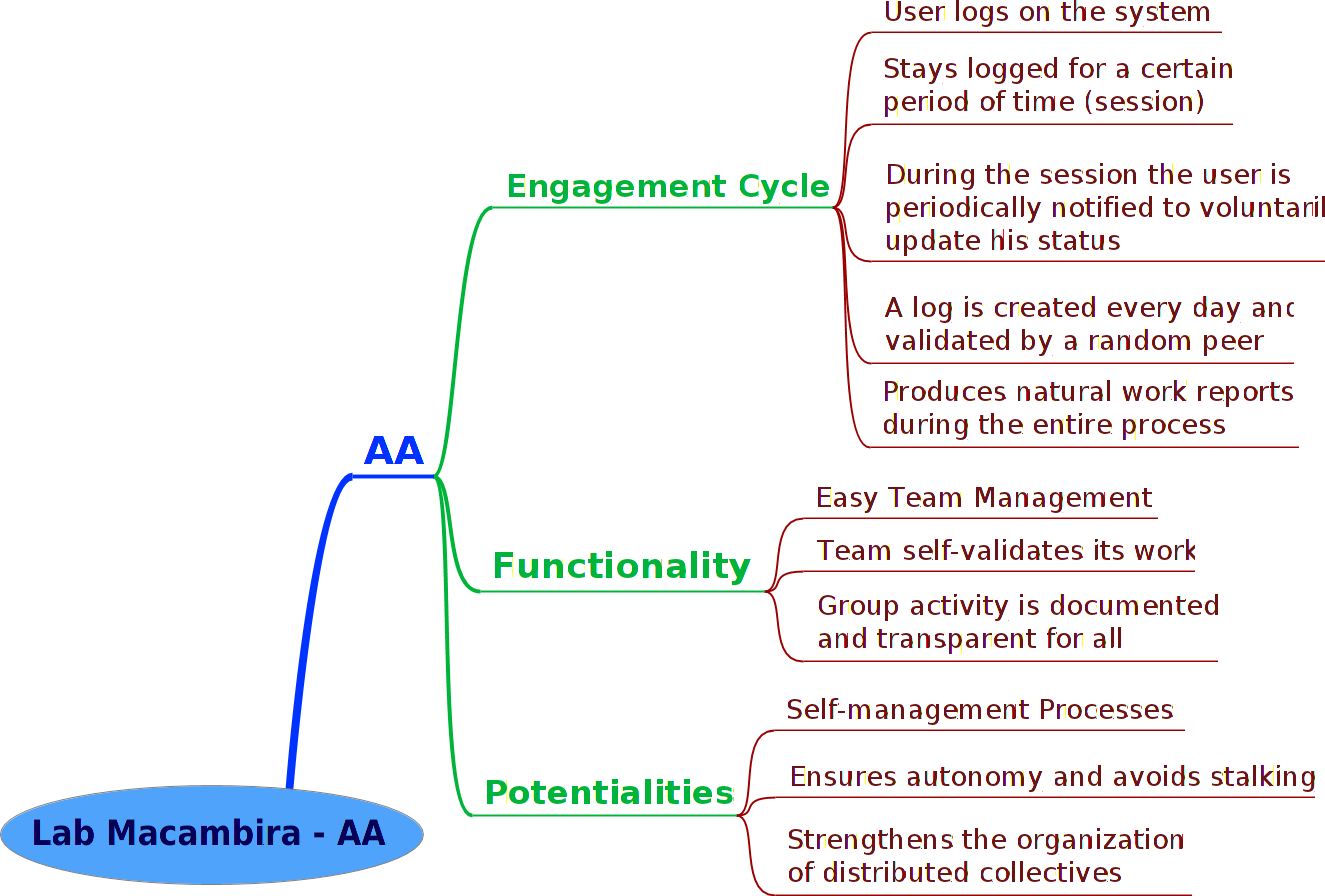
\includegraphics[width=0.8\linewidth,keepaspectratio=true]{figs/aa-mm.png}
\end{center}
   \caption{
   A mindmap of our methodology
   }
\label{fig:mm}
\end{figure}

\subsection{AA Session}

From the developer's perspective, the AA methodology is based on
creating pretty small high perspective reports of what they are doing
in a specific time frame, that can be something between 5 to 15
minutes, depending on what is most convenient for the developer and the team. An
\emph{AA Session} would be a period of at least 2 hours doing these periodical
\emph{micrologs} also called \emph{AA posts}. The developer can set reminders or alerts to show up when its time to
\emph{microlog}. The objective of the flexible time frame and
alert scheme is to \emph{minimize developer overhead} during his AA session. In
this way, the developer can issue micrologs while staying maximally concentrated in his
code. Each microlog may be sent directly to an on-line server, or stored
locally in a temporarily database for sending/pushing later. This enables
offline micrologging and periodical alerting.

Developers optionally record a \emph{video screencast} at the end of the
session summarizing what has been done, explaining with his words and
showing his most important results. This is very similar to the video logging system
in the movie Avatar~\cite{Avatar}, although it is proved from our July 2011 git repositories and online
wiki that we have used this powerful concept in AA prior to the release of
Avatar. Moreover, screencasting differs from general videologging in that it
typically captures actual workflow on
the computer screen. Screencasting, combined with the textual log of the AA
Session, renders the final report more understandable for the individual developer himself
or to other people searching for information about his production.

\subsection{AA Website Report}

\begin{figure}
\begin{center}
   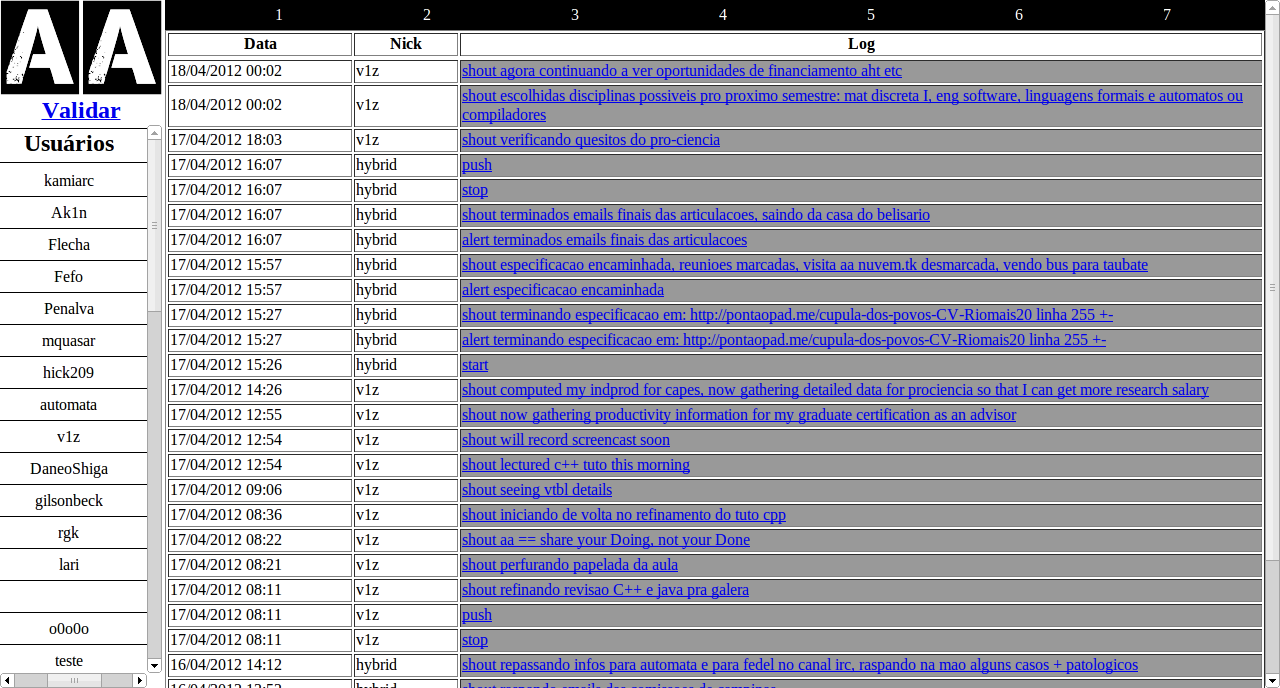
\includegraphics[width=0.95\linewidth]{figs/aa-0_1.png}
\end{center}
   \caption{AA Version 0.1}
\label{fig:aaserver}
\end{figure}

All AA reports made by the developers are ultimatelly sent to a Web server and
become publically aggregated on a Website, enabling a manager or another
developer to follow very closely the work of a given developer, nearly real-time,
reading each of his small reports or micrologs of what he is doing right now.

Another use case is to check older sessions to check when certain tasks
were carried out and the comments of the developer about the \emph{process}.
Since each AA microlog happens in a very short timeframe of work, the information
about what was was done -- specially \emph{how} it was done -- becomes very easy to
understand, instead of a long report in the end of a session.

IN the current version of the AA server infrastructure, the aggregating
website is where the developer can attach a link for his
screencast about each session. Screencasts are specially useful on cases where
the small reports were done in a hurry, because the developer did not want to
lose his focus on something important at that moment.

\subsection{Peer Validation}

In order to prevent spamming and to improve the overall quality of AA reports,
each AA session must be validated by another developer. More specifically,
all reports are read by someone that will mark them as `valid' or `invalid'
and may optionally write commentaries about the specific session and quality of
micrologs. The developer in charge of validating any given session is randomly assigned 
by the AA Web server, which sends an email to the chosen developer with an URL to
a validation interface. 

% TODO: adicionar figura aa cliente (ou tabela com os principais comandos)
% TODO: adicionar figura com arquitetura do AA cliente + AA web + validação
% TODO: melhorar screenshot do AA web

\section{Results and Discussion}
\label{results}

Easy and effective GSD team management is the main
purpose of the AA methodology. We applied the proposed methodology to a group
of 9 developers in July of 2011 on what we called Lab
Macambira~\footnote{LabMacambira.sf.net: \url{http://labmacambira.sf.net}}. The
main objective of the team was to work on an array of strategic free software
projects in the broad audiovisual and web categories,
contributing directly to their development, submitting bug patches or
committing new features to their source code.

The team members had different levels of experience on software
development for large and distributed free software projects
like Scilab or Mozilla. In this way, one month of training was
conducted by two experienced developers, teaching the basics of use of
development support tools like bugtrackers, programming languages,
version control systems, and build systems. After this period, a starter project
was proposed for new developers, namely to have an accepted patch or commit to
the official repository for a large and widely used free software app.
Developers passing the starter project would be deemed `initiated' and be
called a `Macambira' developer.  Table~\ref{tabela:contribuicoes} summarizes the
effective accepted contributions of each successfully initiated developer to
free software projects in 2011.

%% adicionar tabela de contribuições

\begin{table}
  \caption{Free and open software projects that received contributions
    from ``Macambiras''. On the first column we can see a list of
    applications of those projects. At right, the pseudonym of the
    ``Macambiras'' who sent \textit{commits} to the application. At
    ``Lab Macambira'', and at free software community in general, is a
    common practice to use pseudonym as identification.}
    \begin{tabular}{|l|l|}
        \hline
        Application           & ``Commiters''                       \\
        \hline \hline
        Mozilla Firefox       & daneoshiga, bzum                    \\
        Evince                & hick209, bzum, marcicano, mquasar   \\
        BePDF / Xpdf          & marcicano                           \\
        Ekiga                 & flecha                              \\
        Empathy               & fefo                                \\
        Lib Folks (Telepathy) & kamiarc                             \\
        Scilab                & v1z, humannoise                     \\
        VxL                   & v1z                                 \\
        ImageMagick           & v1z                                 \\
        OpenOffice            & hick209                             \\
        Puredata              & v1z, automata, greenkobold, gilson, bzum \\
        Puredata OpenCV       & v1z                                 \\
        Puredata GEM          & v1z, fefo, hick209                  \\
        Puredata PDP          & v1z, fefo, hick209                  \\
        ChucK                 & rfabbri, automata                   \\
        ChucK MiniAudicle     & rfabbri, automata                   \\
        WebRTC                & automata                            \\
        OSC-Web               & automata                            \\
        Web-PD-GUI            & automata                            \\
        Live-Processing       & automata                            \\
        ChucK-Wiimote         & automata                            \\
        Audiolet              & automata                            \\
        Extempore             & automata                            \\
        \hline
    \end{tabular}
    \label{tabela:contribuicoes}
\end{table}

In one month, each developer contributed to many very large free software
projects. Many of the developers started the training with no
knowledge of what is free software and ended that period becoming a
free software developer.

During that month, the same team developed the first version of the AA
system and used AA to manage their activities. Even while developing
the system. All the source code of AA --- the client that sends the
logs and the AA Web server --- is public available~\footnote{AA source
  code:
  \url{http://labmacambira.git.sourceforge.net/git/gitweb.cgi?p=labmacambira/aa}}
and all the AA sessions log of the whole team of ``Lab Macambira'' is
also on-line~\footnote{Logs of AA sessions:
  \url{http://labmacambira.git.sourceforge.net/git/gitweb.cgi?p=labmacambira/paainel}}.

After the training period, during more 6 months, the ``Macambiras''
worked on a large range of free software projects, distributed on work
groups --- each work group focusing on a specific theme like video,
audio and web --- and financed by contracts and support of the
``Pont\~{a}o N\'{o}s Digitais''. In Table~\ref{tabela:criados} we can
see a list of the free software created by ``Lab Macambira'' since
July of 2011.

\begin{table}
    \caption{Software projects created by ``Lab Macambira'' since July
      of 2011 with a short description and the technologies --- like
      programming languages or frameworks --- involved. It is
      interesting to note the heterogeneity of projects and its areas
      of application.}
    \begin{tabular}{|l|p{5cm}|l|}
        \hline
        Application & Description & Technologies involved \\ 
        \hline \hline
        AA            & Algorithmic Auto-regulation      & Python, PHP \\
        \hline
        \'{A}gora Communs & System for on-line deliberations & PHP \\
        \hline
        SIP           & Scilab Image Processing toolbox & C, Scilab \\
        \hline
        animal        & An Imaging Library              & C \\
        \hline
        TeDi          & Test Framework for Distance Transform
        Algorithms & C, Shellscript, Scilab \\
        \hline
        Macambot      & Multi-use IRC Bot               & Python \\
        \hline
        ``Confer\^{e}ncia Permanente'' & Platform for the permanent
        conference of the rights of minors & PHP, JavaScript \\
        \hline
        CPC           & Center for accounting of the Brazilian culture
        representation groups & Python, Django \\
        \hline
        Timeline      & Interactive time lines on the Web & JavaScript
        \\
        \hline
        Imagemap      & Interactive marking for on-line photos &
        JavaScript \\
        \hline
        ABT           & Program for real-time execution and musical
        rhythmic analysis & Python \\
        \hline
        EKP           & Emotional Kernel Panic & Python, ChucK \\
        \hline
        SOS           & Aggregation and diffusion of popular and native
        knowledge about health & Python, Django \\
        \hline
        Creative Economy & Platform for creative, collaborative and
        solidarity economy of the culture hubs and cultural entities &
        Python, Django \\
        \hline
        OpenID Integration & Adaptations to existing software for
        unified login through OpenID & PHP \\
        \hline
        pAAinel & Dashboard for the real-time visualization of Lab
        Macambira activity & Python, Django \\
        \hline
        Georef & Collection of scripts to be used as reference, which
        aims to be a GIS platform to map public data of use to
        citizens & Python, Django \\
        \hline
        AirHackTable & Software for an instrument which generates
        sound from flying origami tracked by webcams & Puredata,
        C/C++, Scilab \\
        \hline
        \end{tabular}
    \label{tabela:criados}
\end{table}

As of this writing the ``Lab Macambira'' have many software
developers, and some of the trained developers continue to work
voluntarily in the project.

\section{Conclusions}
\label{conclusions}

%% brief introduction
In a scenario where GCD is growing as a popular form of software
development, not just on free software projects but in the whole
software industry, we need methodologies to deal with its
disadvantages and at the same time to amplify its advantages.

This paper has presented a methodology to GCD, being the development
conducted on large or small groups of software developers, working on
different countries or even at the same room. The AA methodology
implements a simple system where each developer take notes of his work
generating a periodical log of small text sentences. The sum of those
sentences, along an entire session of work, results in a complete
report. The report is made public available through a Website and be
validated by other developers sorted aleatory by the AA Web server.

Instead of a merely work-management tool, AA act as a methodology to
improve the time sense of individuals, dividing their work on small
sessions, and also reducing the need of extensive
reports or unnecessary meetings. By asking users to write a minimal
text sentence as a continuously log, AA does not disturb developers
concentrated on programming: developers just have to type some
characters, hit \textit{enter} and go back to coding.

AA application is not restricted to software development. As of this
writing there is a comic book studio~\footnote{Pula pirata:
  \url{http://pulapirata.com}} starting to use AA to manage their
activities. People with non-software background, like social
scientists, musicians and activists has also using AA and contributing
for its improvement.

For developer teams, we have experienced the use of AA to
auto-regulate the work of ``Lab Macambira'', a group of free software
developers from Brazil. Since July of 2011 the group have contributed
and created new free and open source software for a vast number of
applications.

There are many aspects of the work which remain unfinished. New ways
to report logs --- the ``Twitter like'' messages --- from different
interfaces like IRC, Internet Messaging services and email can make
the use of AA easy and widespread, turning AA an ubiquitous system,
presented on everyday communication channels. Even the work logs
generated since July of 2011 could be vastly statistically analyzed
aiming to recognize patterns in the behavior of individuals and their
productions.

We would like to conclude setting an important role of AA: being a
free software system and an open methodology, AA could be used to
auto-manage groups of individuals working on software or other kinds
of activities. In this way, we are interested to spread AA for those
groups, to have even more developers contributing in a collaborative
way.

\section*{Acknowledgments}
%The authors would like to thank NSF and CNPq.

We would like to also thank AA: the present research and even this
manuscript was written using AA. The complete log is on-line at
\url{http://www.pulapirata.com/skills/aa}.


\nocite{last2003}
\nocite{german2003}
\nocite{carmel1999}
\nocite{carmel2001}
\nocite{komi2005}
\nocite{battin2001}

%{\small
%\input{paper-draft.bbl}
%%%%\bibliographystyle{splncs}
% this is a good style for drafting
%\bibliographystyle{abstract}
% this is a good style for finals
\bibliographystyle{acm}
\bibliography{aa.bib}
%}

\end{document}
